
\section{ Measurable Spaces}
	\label{s:sys}
% The aim of this section is to formalise the main operations we can do on probability spaces. I need to 1) Set the notations on $\Omega$ for the random variables 2) Consider a common sample
% space for two experiments.
	In this Section we continue the discussion started in Subsection~\ref{ss:subset}???? on the structure of sample spaces. Recall that the choice of $\mathfrak F$ determines the elementary events, and, therefore, the sample space $\Omega= \{\omega_1, \ldots, \omega_n\}$. We want to refine the sample space by considering more events, say $\mathfrak F' \supset \mathfrak F$, and this leads to a bigger sample space $\Omega = \{\omega_1, \ldots, \omega_m\}$, with $m > n$. Each elementary event $\omega_i$ in $\Omega$ is an event in $\Omega'$, which can therefore be decomposed, and we can associate to each elementary event in $\Omega'$ the event $\omega_i$ to which it belong. The idea to have in mind is the one of Example~\ref{ex:shop}??? and Figure~\ref{}???, and in this section we proceed in formalising this procedure. $\Omega$ is said to be a refinement of $\Lambda$, or $\Lambda$ a coarse grained version of $\Omega$ depending what we want to stress. Notice that we have already used implicitely a big refinement when writing a Venn diagram for events, see Figure~\ref{}, since the points of the square can be thought as the points of a big, very precise sample space $\Omega$. \\
	The main way in which we will use refinements is to give a common framework when lookig at two different sample spaces jointly.\\
	 On the other side, we will use \emph{coarse grained} version of the sample space $\Omega$ when it will be useful to consider a big, very precise, sample space $\Omega$ that contains all the variables that affect the system we are looking at and which is unknown to us. The probability comes from $\Omega$ and we can observe only a part of it through, for instance,  random variables, see Definition~\ref{}???.   

\subsection{ Coarse Graining and Refinements of Sample Spaces}
	The idea is the following. 
	\begin{definition}
		A pair of $(\Omega, \mathfrak F)$, where $\Omega$ is a discrete space and $\mathfrak F$ is a set of subsets of $\Omega$ closed under intersection.  
	\end{definition}
	Let $\Omega' = \{\omega'_1, \ldots, \omega_m'\}$ be a finite ( but everything can be adapted to the non-discrete case) sample space to be thought large. Conisder a smaller sample space $\Omega =\{\omega_1 , \ldots, \omega_n\}$, $n < m$, and assume that each $\omega_i$ is an event in $\Omega'$, that is, it can be written using the elementary events in $\Omega'$. The example to have in mind is Example~\ref{e}, and Example~\ref{e}.    
	\begin{definition}
		\label{d:restriction}
		A map $\Omega$ together with a surjective function $f: \Omega' \to \Omega$ is said to be a restriction of $\Omega'$. 
	\end{definition}
	\commento{We are omitting a condition, which is fundamental but technical. The events we want to consider in $\Omega$ are also events that we want to consider in $\Omega'$. That is, for all $A \in \mathfrak F$, $f^{-1}(A) \in \mathfrak F'$. This is guaranteed if $\Omega'$ is discrete, but is real condition in the other cases. For fixed $\mathfrak F'$ and $\mathfrak F'$, an $f$ with such property is called $\mathfrak F .\mathfrak F'$ measurable.}

	The meaning of the function $f$ is to associate to each elementary event $\omega' \in \Omega'$, the only event in $\Omega$ to which it is favourable. The next example will help to visualize the concept
	\begin{example}[Two dice]
		\label{ex:two_dice_sample}
		In Example~\ref{ex:sum_restriction} we have considered the same event, two dice that have been or will be rolled, under two different levels of precision. The refined sample space, which considers the face shown by each die, is $\Omega' = \{11,12,13,...,66\}$ and the coarse grained sample space that looks only at the sum is $\Omega = \{2,3,4,\ldots, 12\}$. The function $f$ associates to each result in $\Omega'$ what we observe if we are using $\Omega$, that is, to each pair $ij$, $i,j  = 1,\ldots, 6$, their sum $i + j$: $f(ij ) = i + j $. The function $f$ is represented graphically in Figure~\ref{f:two_dice_sum}.  
	\end{example}

	Consider a restriction $f:\Omega' \to \Omega$. The function $f$ maps the elementary events in $\Omega'$ to the elementary event in $\Omega$ that contains it. The elementary event $\omega$ when seen using $\Omega'$ corresponds to the event 
	\begin{equation}
		\label{e:push_forward}
			f^{-1}(\{\omega\})  = \{\omega' \in \Omega' \,,\, f(\omega' ) = \omega\}.
	\end{equation}
	The next two examples show that Definition~\ref{d:restriction_sample} is often used in the following way:  $\Omega'$ is a big sample space, unknown to us, from which the randomness comes from, and, to evaluate the probabilities in $\Omega$ we need to rewrite the elementary events in terms of $\Omega'$ 
	\bel{}{
		f^{-1}(\{\omega\}) = \{\omega' \in \Omega' \, , \, f(\omega' ) = \omega \},
	}  
	and we will often omit the reference to the large sample by writing the above event as 
	\bel{}{
		(f = \omega).
	}
	In Example~\ref{ex:sum_restriction}, $(f = 5 ) = \{14, 23,32,41\}$, for instance.  
	\begin{example}
		\label{ex:computer}
			Given $p \in [0,1]$ the R function rbinom(1,1,p) gives you a number which can be either $0$ or $1$. It can therefore be regarded as a coin toss with sample space $\Omega = \{0,1\}$. The computer is a deterministic machine and given a sample space $\Omega'$ that describes all the possible states of the computer, including, in particular, the electric current to which the microchips are subjected to used to generate random numbers, should be able to say what is the number generated by the computer. There exists, thereofore, a deterministic function 
	\begin{equation}
	\label{e:restr1}
		\begin{array}{ccc}
			X: & \Omega' \to &  [0,1]\\
			 \omega & \to &  X(\omega ),
		\end{array}
	\end{equation}
	where $X(\omega)$ denotes the number generated by the computer if it were at state $\omega$. If we are interested only in the value this number takes, $\Omega = [0,1]$ and \eqref{e:restr1} is defines a restriction in the sense of Definition~\ref{d:restriction}.  
% Also the function should be random, but we can place the randomness of on the function on the sample space. 
	\end{example}
	
	\begin{example}[Random Variables ]
		\label{ex:random_variable}
		Let $\Omega'$ be a big sample space that considers all the possible values of the possible variables that influence the object you are looking at. If looking at a coin toss it could contain the position of the coin at the moment of being tossed, the force we gave to it, variables describing the wind strength, the personality of the person tossing it... It si mostly unknown and the randomness comes okn that space because of this. usually from that big sample space  
		A particular way to measure the 
		We are interested in events of the form $[a, b]$, where $a \leq b$.  
	\end{example}


	\subsection{Common Sample Spaces and Cartesian Product}
	% The cartesian product is minimal in the following categorical sense: every other extension contains the cartesian product... But what about $X\times X$? Should I ask something about the sigma algebras generated by the two extnsions 
	When performing two different experiment it is necessaty to have a common sample space that considers them at the same time. In this section we use the letter $\Gamma$ for the large sample space $\Omega'$ and we consider two experiments $\Omega = \{\omega_1, \ldots, \omega_n\}$ and $\Lambda = \{\lambda_1, \ldots, \lambda_m\}$, for some $m,n \in \mathbb N$. 
	\begin{definition}
		A common refinement of $ \Omega$ and $\Lambda$ is a sample space $\Gamma$ and two surjective functions $f:\Gamma \to \Omega$ and $g:\Gamma \to \Lambda$ that form a refinement for $\Omega$ and $\Lambda$, respectively.  said to be a joint realization of $\Omega$ and $\Lambda$
	\end{definition}
	Working on a sample space which is finer than $\Omega$ and $\Lambda$ is necessary to do a probabilistic analysis of the outcomes in $\Omega$ and $\Lambda$ when considered toghether. Fortunately, there is a standard way to build a "minimal" (in some sense) a refinement $\Gamma$ of both  $\Omega$ and $\Lambda$. 
	\begin{example}
		\label{ex:cartesian_product}
		Let $\Omega$ and $\Lambda$ be two sample spaces as above and consider the cartesian product of $\Omega$ and $\Lambda$, which is the set of two digit strind where ther first digit is an element of $\Omega$ and the second one an element of $\Lambda$, 
		\begin{equation}
				\label{e:cartesian_product}
				\Gamma = \Omega \times \Lambda =\{\omega\lambda\,,\omega \in \Omega, \lambda \in \Lambda\} = \{\omega_1 \lambda_1 ,\ldots, \omega_n\lambda_m\}.
		\end{equation}
		Consider also the coordinate functions $\omega: \Omega \times \Lambda\to \Omega$ and $\lambda = \Omega \times \Lambda \to \Lambda$, defined by $\omega(\omega_i \lambda_j )  = \omega_i$ and $\lambda(\omega_i \lambda_j) = \lambda_j$, respectively. Then $\Gamma := \Omega \times \Lambda$ together with $\omega: \Gamma \to \Omega$ and $\lambda: \Gamma \to \Lambda$ is a common refinement of $\Omega$ and $\Gamma$. \\
		The marginal sets 
		\begin{equation}
			\label{e:marginal}
			\begin{split}
				(\omega = \omega_j) & := \{\omega\eta \in \Omega \times \Lambda\,, omega = \omega_i\} = \{\omega_1\lambda, \ldots, \omega_m\lambda_j\}\\
				(\lambda = \lambda_j) & : = \{ \omega\eta \in \Omega\times \Lambda \, \lambda = \lambda_j\} = \{\omega_1\lambda_j,\ldots , \omega_n \lambda_j\}
			\end{split}
		\end{equation}
		are depicted in Figure~\ref{f}  \ref{f} and \ref{} for each $i = 1,\ldots, n$ and $j = 1,\ldots, m$. 
	\end{example}
	not anymore elementary when looked in $\Omega'$, since the set $\{\}$ elElementary events in $\Omega$ are not longer elementary w
	
\begin{figure}[h]
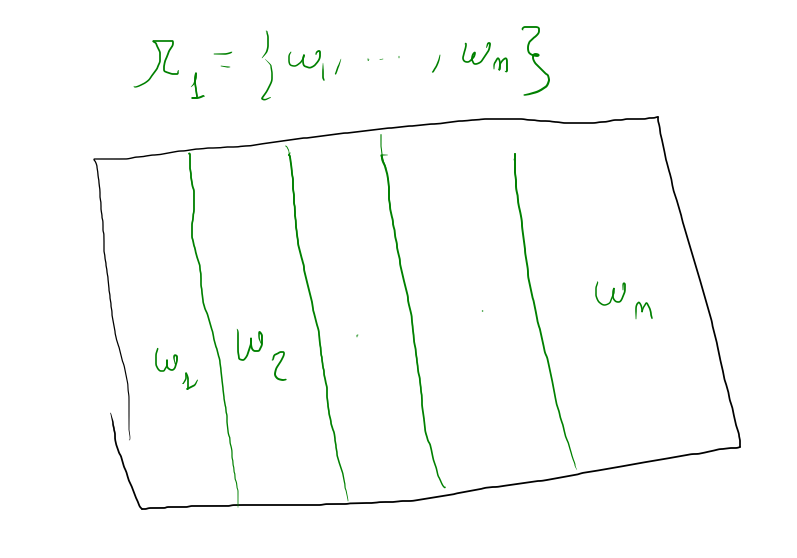
\includegraphics[width = 12cm]{First_marginal.png}
\label{f:omega}
\end{figure}
\begin{figure}[h]
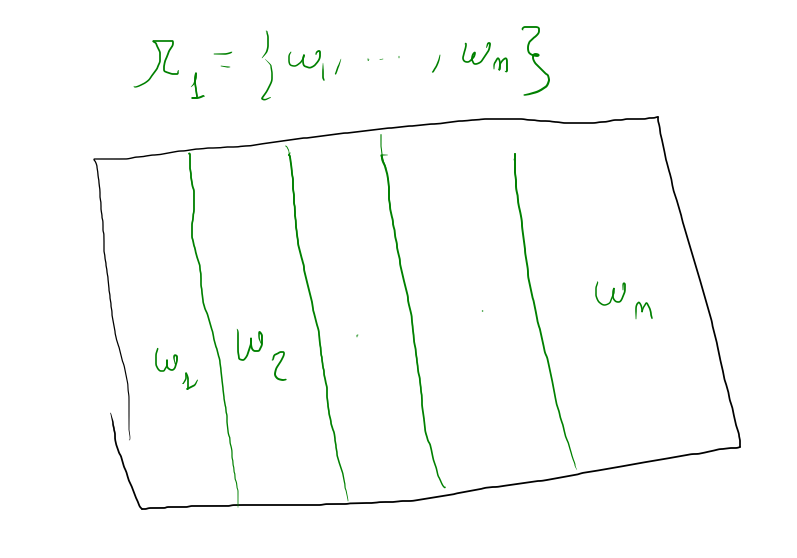
\includegraphics[width = 12cm]{First_marginal.png}
\label{f:second}
\end{figure}
\begin{figure}[h]
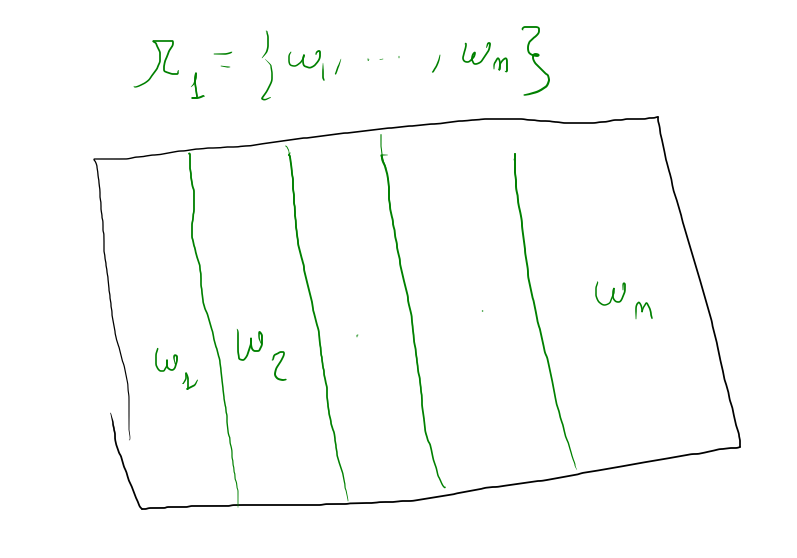
\includegraphics[width = 12cm]{First_marginal.png}
\label{f:product}
\end{figure}

	\begin{example}[Two Random Variables]
		\label{ex:joint_sample}
		Two random variables $X,Y$ defined on the same measurable space $\Omega$ are 
	\end{example}

\begin{ExerciseList}

\Exercise How many elements does $\Omega\times \Lambda$ have?
\Answer $n\times m $. To see this, note that for each $i=1,..,n$ there are $m$ different elementary events: $(\omega_i,\eta_1),...(\omega_i,\eta_m)$. For every $i$ which varies from 1 to $n$, we have $m$ different elements.
i
\end{ExerciseList}
	\begin{figure}[h]
		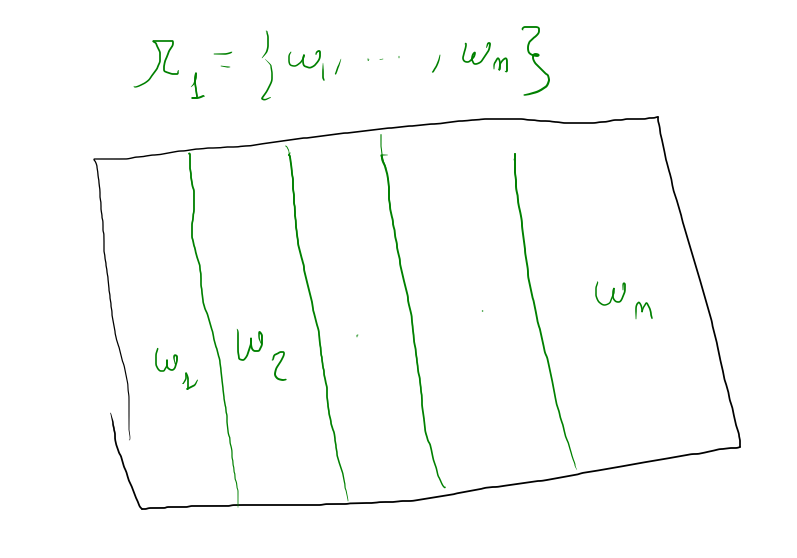
\includegraphics{First_marginal.png}
		\caption{ The sample space of one coin toss \label{f:1marginal}}
	\end{figure}

	
	\begin{figure}[h]
		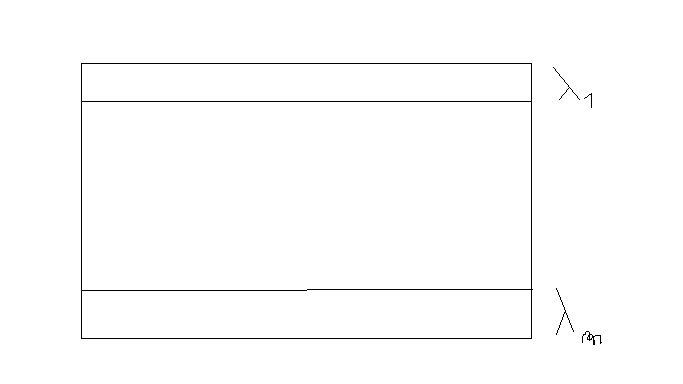
\includegraphics{Second_marginal.png}
		\caption{ The sample space of one coin toss \label{f:2marginal}}
	\end{figure}

	\begin{figure}[h]
		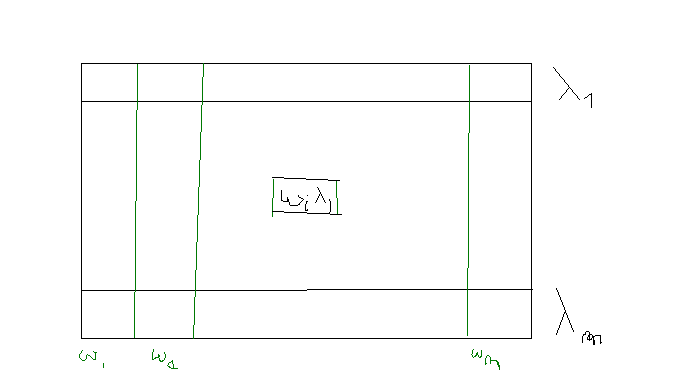
\includegraphics{Cartesian_product1.png}
		\caption{ The sample space of one coin toss \label{f:cartesian}}
	\end{figure}



